%iffalse
\let\negmedspace\undefined
\let\negthickspace\undefined
\documentclass[journal,12pt,onecolumn]{IEEEtran}
\usepackage{cite}
\usepackage{amsmath,amssymb,amsfonts,amsthm}
\usepackage{algorithmic}
\usepackage{multicol}
\usepackage{graphicx}
\usepackage{textcomp}
\usepackage{xcolor}
\usepackage{txfonts}
\usepackage{listings}
\usepackage{enumitem}
\usepackage{mathtools}
\usepackage{gensymb}
\usepackage{comment}
\usepackage[breaklinks=true]{hyperref}
\usepackage{tkz-euclide} 
\usepackage{listings}
\usepackage{gvv}                                        
%\def\inputGnumericTable{}                                 
\usepackage[latin1]{inputenc}                                
\usepackage{color}                                            
\usepackage{array}                                            
\usepackage{longtable}                                       
\usepackage{calc}                                             
\usepackage{multirow}                                         
\usepackage{hhline}                                           
\usepackage{ifthen}                                           
\usepackage{lscape}
\usepackage{tabularx}
\usepackage{array}
\usepackage{float}
\newtheorem{theorem}{Theorem}[section]
\newtheorem{problem}{Problem}
\newtheorem{proposition}{Proposition}[section]
\newtheorem{lemma}{Lemma}[section]
\newtheorem{corollary}[theorem]{Corollary}
\newtheorem{example}{Example}[section]
\newtheorem{definition}[problem]{Definition}
\newcommand{\BEQA}{\begin{eqnarray}}
\newcommand{\EEQA}{\end{eqnarray}}
\newcommand{\define}{\stackrel{\triangle}{=}}
\theoremstyle{remark}
\newtheorem{rem}{Remark}

% Marks the beginning of the document
\begin{document}
\bibliographystyle{IEEEtran}
\vspace{3cm}

\title{\textbf{NCERT 9.4.3}}
\author{EE24BTECH11032- John Bobby}
\maketitle
\bigskip
\textbf{Question:} Find the solution for the differential equation $\frac{dy}{dx}+y=1$\\
\section{Mathematical Approach} 
\begin{align*}
    \frac{dy}{dx}=1-y\\
\end{align*}
On rearranging the terms,
\begin{align*}
    \frac{dy}{1-y}&=dx\\
    \int \frac{dy}{1-y}&=\int dx\\
    -\log{\abs{y-1}}+c_1&=x+c_2
\end{align*}
On simplification 
\begin{align*}
    -\log{\abs{y-1}}=x+c\\
    \abs{y-1}=\pm e^{-x}\\
    y=1\pm e^{-x}\\
\end{align*}
For the numerical approach we are assuming that the function passes through origin\\
Thus is the function $y$ is,
\begin{align*}
    y=1-e^{-x}
\end{align*}
\section{Laplace Transform}
Take the Laplace transform of both sides,\\
\begin{align*}
    \mathcal{L}\left\{\frac{dy}{dx}\right\} = \mathcal{L}\{1 - y\}
\end{align*}
Using the Laplace transform properties,\\
\begin{align*}
    \mathcal{L}\left\{\frac{dy}{dx}\right\} = sY(s) - y(0), \quad \mathcal{L}\{1\} = \frac{1}{s}, \quad \mathcal{L}\{y(t)\} = Y(s)\\
\end{align*}
On rearranging,\\
\begin{align*}
    sY(s) - y(0) = \frac{1}{s} - Y(s)\\
    sY(s) + Y(s) = \frac{1}{s} + y(0)\\
    Y(s)(s + 1) = \frac{1}{s} + y(0)\\
    Y(s) = \frac{1}{s(s+1)} + \frac{y(0)}{s+1}
\end{align*}
Taking the inverse laplace transform \\
\begin{align*}
\mathcal{L}^{-1}\brak{Y\brak{s}}=y\brak{x}\\
    \mathcal{L}^{-1}\brak{\frac{1}{s\brak{s+1}}}=1-e^{-x}\\
    \mathcal{L}^{-1}\brak{\frac{y\brak{0}}{s+1}}=y\brak{0}e^{-x}\\
    y\brak{x}=1-e^{-x}+y\brak{0}e^{-x}\\
\end{align*}
As $y\brak{0}=0$
The solution is 
\begin{align*}
    y\brak{x}=1-e^{-x}
\end{align*}
\section{Z Transform}
\begin{align*}
  \frac{dy}{dx}=\frac{{}y_{n+1}-y_{n}}{h}\\
  y_{n+1}=y_{n}+\frac{dy}{dx}h\\
  y_{n+1}=y_{n}+\brak{1-y_{n}}h\\
\end{align*}
Applying Z Transform on both sides\\
\begin{align*}
    \mathcal{Z}\{y(k+1)\} = z.Y\brak{z}-z.y\brak{0}\\
    \mathcal{Z}\{y(k)\}=Y\brak{z}\\
    \mathcal{Z}\{1-y(k)\}=\frac{1}{1-z^{-1}}-Y\brak{z}\\
    z Y(z) - z y(0) = Y(z) + h \left( \frac{1}{1 - z^{-1}} - Y(z) \right)\\
\end{align*}
Solving for $Y\brak{z}$,\\
\begin{align*}
    Y(z) = \frac{z y(0) + h}{z - 1 + h}=\frac{h}{z - 1 + h} \quad \brak{y\brak{0}=0}
\end{align*}
Applying Z Inverse,
\begin{align*}
y\brak{x}=h(1-h)^{x}u\sbrak{x}
\end{align*}
\section{Numerical Approach}
\begin{align*}
\frac{dy}{dx}=\lim_{h \rightarrow 0} \frac{y\brak{x+h}-y\brak{x}}{h}
=\lim_{h \rightarrow 0}\frac{{}y_{n+1}-y_{n}}{h}
\end{align*}

If $h$ is sufficiently small,\\
\begin{align*}
  \frac{dy}{dx}=\frac{{}y_{n+1}-y_{n}}{h}\\
  y_{n+1}=y_{n}+\frac{dy}{dx}h\\
  y_{n+1}=y_{n}+\brak{1-y_{n}}h\\
\end{align*}
Thus the value of $y_{n+1}$ can be predicted if we know the value of $y_{n}$\\
For this question 
\begin{enumerate}
    \item The interval $\sbrak{0,5}$ is divided  into $51$ equal parts each of width $0.1$units
    \item On starting from a known point $\brak{x,y}$ the value for $y\brak{x+0.1}$ is calculated. This procedure is repeated until the value of $x$ reaches $5$.
    \item Knowing all the $y$ values for the equally spaced $x$ values in interval, the solution plot can be plotted.
\end{enumerate}
\newpage
The plot is given below\\
\begin{figure}[h!]
    \centering
    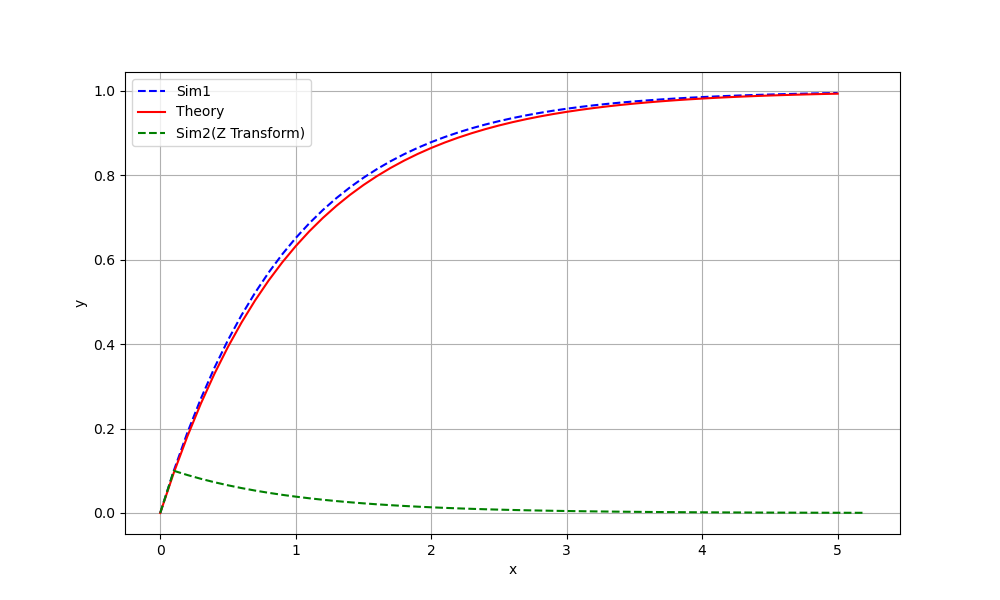
\includegraphics[width=0.7\columnwidth]{figs/Q1.png}
    \label{stemplot}
\end{figure}






\end{document}
